\documentclass{report}

\usepackage{geometry}
\usepackage{verbatim}
\usepackage[table]{xcolor}
\usepackage{subcaption}
\usepackage{graphicx}

\begin{document}

\chapter{Introduction}

The computing infrastructure that underpins today's world is insecure. Code written
in unsafe languages (e.g., C) may hide any number of programming bugs that go uncaught
until they are exploited in the wild, especially memory errors. Safe or not, any code
might contain logic errors (SQL injection, input-sanitization flaws, etc.) that subvert
its security requirements.

Although static analyses can detect and mitigate many insecurities, an important line of
defense against undetected or unfixable vulnerabilities is runtime enforcement of
{\em security policies} using a reference monitor~\cite{Anderson72:PlanningStudy}.
A security policy restricts the behavior of the system, typically by interrupting
a badly-behaved process, termed ``failstop behavior.'' At the most general, a policy could be
any kind of runtime check, from simple assertions (``at line X, variable Y has value Z'') to
sophisticated temporal logic formulae.

This dissertation focuses on a class of policies that can be specified in terms of flow constraints
on \emph{metadata tags}. A tag annotates a value with information like type, provenance,
ownership, or security classification, and a tag-based policy is defined solely in terms of
the interaction of tags, without reference to the values that they are attached to.
Notable policies that can be implemented in this way include:

\begin{itemize}
\item {\em Memory safety}, which restricts programs in memory unsafe languages to obey
  the spatial and/or temporal constraints of the language, turning unchecked errors into
  checked ones
\item {\em Information flow control} (IFC), in which data identified as being in some way secret
  or sensitive is preventing from leaking on an externally visible
\item {\em Compartmentalization}, in which programs are divided into components (compartments)
  with restricted access to data and other resources
\item {\em Mandatory access control}, which identifies ``subjects'' (possibly compartments,
  but also non-code entities such as users) and explicitly restricts their access to resources
\end{itemize}

Tag-based policies include a number of important security concepts, and are well-suited to
efficient hardware enforcement. As an exemplar of hardware tag monitors, take the 
PIPE\footnote{ Variants of PIPE have
been called PUMP~\cite{Dhawan+15} or SDMP~\cite{RoesslerD18} and marketed commercially
under the names Dover CoreGuard and Draper Inherently Secure Processor.}
(Processor Interlocks for Policy Enforcement) ISA extension \cite{Azevedo+16,Azevedo+15}.

PIPE is a programmable hardware mechanism that associates large (word-sized) metadata tags
with every word of memory and register. At each step of execution, while the ALU processes
the operands of the current instruction, the tags associated with those operands are processed
by a module called the ``tag management unit'' (TMU).
The TMU, instantiated as a cache or lookup table into a set of software-defined rules,
consults those rules to (1) determine whether the operation should
proceed, sending an interrupt if not, and (2) compute updated tags to associate with the
outputs of the operation. These rules collectively define a state machine operating on the
tags in the system, which is termed a ``micro-policy,'' a concrete instantiation of the
sorts of policies mentioned above.

Because PIPE tags are so large, they can encode complex data structures, giving PIPE a high
degree of flexibility in the policies that it can enforce. It is even feasible to layer
multiple policies on top of one another by taking the Cartesian product of their tags.
And because tags are inaccessible to normal execution, PIPE policies are protected from
subversion by application code.

However, the complexity of PIPE's style of tagging leads to challenges in the definition,
specification, and verification of policies, demonstrated via several examples.
This dissertation addresses those challenges.

\paragraph{Example: Spatial Stack Safety}

Tag policies are difficult to write.
A policy consists of a collection of rules, each associated with a family of opcodes.
Almost all policies will need to distinguish
individual special instructions via tags on their values in memory, since many opcodes can
play different roles that need to be
treated differently in the policy. Defining a policy requires knowledge of both the assembly
language of the host ISA and the behavior of the compiler, so that the policy designer can
identify which instructions serve special purposes. Many policies require the binary
to be rewritten with additional instructions whose primary purpose is moving and manipulating
tags.

For example, Figure \ref{ex:call} shows how a single function header must be updated to
support a (simplified) spatial stack safety policy. The purpose of this policy is to prevent
loads and stores to stack frames other than that of the active function.
The policy is conceptually simple:
each location in a stack frame is identified by the depth of the frame, and the stack pointer
is tagged with the depth of the current function.  Loads and stores of stack
addresses must use a pointer that matches that of the location, i.e. the current stack pointer
or a pointer derived from it. For simplicity, this version does not attempt to protect deallocated
frames (which may share the depth of the active frame), so it only offers spatial and not temporal
protection.

Figure \ref{ex:call1} shows a typical header sequence in assembly for a function whose frame
(including saved return address) is sixteen bytes. It simply allocates those bytes by decreasing
the stack pointer, then stores the return address to the stack. Later it will attempt to store data
elsewhere in the frame, then load it. Figure \ref{ex:call2} gives a sense of how
this code might be instrumented with tags, and Figure \ref{ex:call3} describes some of
the rules that act on these tags. The header sequence is given special tags to enforce
that it runs from beginning to end and only following a call, and instructions are added
to initialize tags on the stack frame.

A significant portion of the policy's rules is dedicated to bookkeeping, in this case
mostly for purposes of ensuring that the header sequence executes in order (red).
Only the lines in blue deal with the main focus of the policy:
tagging the frame and the stack pointer with the current depth of the call stack, and enforcing
that a stack address can only be written through the stack pointer at the same depth.

Security policies are challenging to write, and subtle errors can enable them to be compromised.
It is therefore vital that they be validated. But first they must be specified. What does the
policy actually set out to do? What protection does it offer? In the interest of simplicity,
this example only offered spatial, not temporal, safety. If it were meant to be more than
an illustrative example, spatial stack safety should be formally defined so that the policy can be
shown to enforce it. Then it will be up to the user whether that level of security is sufficient.

This is a common problem for more realistic policies, as well.
In many cases, there is no standard specification for the kind of security that a policy hopes
to enforce. Even in cases where there is an existing formal specification, such as
memory safety \cite{Azevedo+16}, trade-offs between performance and protection may result in a
policy that does not precisely match it. In these cases, the policy needs to be specified so
that its purpose is clear.

Once defined and specified, a policy needs to be validated, either by testing or formal verification.
Verification is preferable, as proofs rule out the possibility of bugs too subtle to show up in testing.
But randomized property-based testing can increase confidence in a policy when proof is infeasible.
Regardless of which validation method, it is valuable to define, specify, and validate a policy,
adding one more tool to the developer's security kit.

\begin{figure}
  \begin{subfigure}[t]{0.55\textwidth}
    \vspace{0em}
    \begin{tabular}{l l}
      0: {\tt sub sp 16 sp} & Allocate sixteen bytes \\
      8: {\tt store ra sp} & Save return address \\
      \dots \\
      32: {\tt store 42 (sp+8)} & Store to stack in body \\
      \dots \\
      64: {\tt load r0 (sp+8)} & Load from stack in body \\
    \end{tabular}
    \caption{Initial generated code}
    \label{ex:call1}
  \end{subfigure}
  \begin{subfigure}[t]{0.45\textwidth}
    \vspace{0em}
    \begin{tabular}{l l}
      0: {\tt sub sp 16 sp} & @ {\sc Head}\((0)\) \\
      8: {\tt store ra sp} & @ {\sc Head}\((1)\) \\
      16: {\tt store 0 (sp+8)} & @ {\sc Head}\((2)\) \\
      24: {\tt nop} & @ {\sc Entry} \\
      \dots \\
      48: {\tt store 42 (sp+8)} & @ {\sc Normal} \\
      \dots \\
      80: {\tt load r0 (sp+8)} & @ {\sc Normal} \\
    \end{tabular}
    \caption{Code tagged and expanded for policy}
    \label{ex:call2}
  \end{subfigure}

  \vspace{\belowdisplayskip}
  
  \begin{subfigure}{\textwidth}
    \begin{tabular}{|l|}
      \hline
      When executing {\tt sub imm r}@{\sc Head}\((0)\): \\
      \hline
      \rowcolor{red!20}
      \(\cdot\) Preceding instruction must have tag {\sc Call} \\
      \rowcolor{blue!30}
      \(\cdot\) Tag on {\tt r} must be {\sc Depth}\((n)\) for some \(n\) \\
      \rowcolor{blue!30}
      \(\cdot\) Set tag on {\tt r} to {\sc Depth}\((n+1)\) \\
      \hline
    \end{tabular}
    %
   \begin{tabular}{|l|}
      \hline
      When executing {\tt store r1 r2}@{\sc Head}\((1)\): \\
      \hline
      \rowcolor{red!20}
      \(\cdot\) Preceding instruction must have tag {\sc Head}\((0)\) \\
      \rowcolor{red!20}
      \(\cdot\) Set tag at {\tt r2}'s target to {\sc RetPtr} \\
      \hline
    \end{tabular}
    
    \begin{tabular}{|l|}
      \hline
      When executing {\tt store imm (r+x)}@{\sc Head}\((n)\): \\
      \hline
      \rowcolor{red!20}
      \(\cdot\) Preceding instruction must have tag {\sc Head}\((n-1)\) \\
      \rowcolor{blue!30}
      \(\cdot\) Tag on {\tt r} must be {\sc Depth}\((m)\) \\
      \rowcolor{blue!30}
      \(\cdot\) Set tag at {\tt r}'s target to {\sc Depth}\((m)\) \\
      \hline
    \end{tabular}
    %
    \begin{tabular}{|l|}
      \hline
      When executing \(\underline{~~}\)@{\sc Entry} \\
      \hline
      \rowcolor{red!20}
      \(\cdot\) Preceding instruction must have tag \\
      \rowcolor{red!20} {\sc Head}\((size / 8)\) \\
      \hline
    \end{tabular}
    
    \begin{tabular}{|l|}
      \hline
      When executing {\tt load \_ (r+x)}@{\sc Normal} \\
      \hline
      \rowcolor{blue!30}
      \(\cdot\) If tag on {\tt r}'s target is {\sc Depth}\((m)\), then
      tag on {\tt r} must be tagged {\sc Depth}\((m)\) \\
      \hline
    \end{tabular}
    
    \begin{tabular}{|l|}
      \hline
      When executing {\tt store \_ (r+x)}@{\sc Normal} \\
      \hline
      \rowcolor{blue!30}
      \(\cdot\) If tag on {\tt r}'s target is {\sc Depth}\((m)\), then
      tag on {\tt r} must be tagged {\sc Depth}\((m)\) \\
      \hline
    \end{tabular}
    \caption{Associated policy rules}
    \label{ex:call3}
  \end{subfigure}

  \caption{Example: Adding Stack Safety policy at call}
  \label{ex:call}
\end{figure}

\paragraph{IFC}

The example in Figure \ref{ex:if} illustrates another scenario that requires the assembly to be
rewritten. An important class of ``information flow control'' (IFC) policies needs to keep track
of when execution is in a state that depends on a secret value. In the source snippet in \ref{ex:if0},
the choice of whether execution reaches line 3 depends on the value of {\tt x},
but it will always reach line 5 regardless of {\tt x}.

Policies typically track contextual information about the current control flow via the tag on
the program counter. In this case, the program counter needs to be updated inside of the {\tt if}
block and then restored to its old value once it leaves. In the expanded code in Figure \ref{ex:if2},
the subtraction instruction at 16 saves a zero tagged with the program counter's tag to {\tt r2}.
Then, at the join point at 40, the jump instruction has no effect except that it enables the policy
to restore the tag on {\tt r2} to the program counter.

These modifications can be automated at the assembly level, given relevant annotations from
the compiler, but the process amounts to an ad hoc compiler pass. It would be better to do it within
the compiler! Then the compiler can handle most of the bookkeeping, leaving the policy developer free
to focus on the rules that are relevant to the policy at hand.

\begin{figure}
  \begin{subfigure}[t]{0.22\textwidth}
    \vspace{0em}
    {\tt 1: int x, y;

    2: if (x == 42) \{

    3: ~~~ y = 0;

    4: \}

    5: x = 0;
    }

    \caption{Source program}
    \label{ex:if0}
  \end{subfigure}
  \begin{subfigure}[t]{0.42\textwidth}
    \vspace{0em}
    \begin{tabular}{l l}
      0: {\tt load r0 (sp+8)} & Load {\tt x} \\
      8: {\tt add zero 42 r1} & Constant 42 \\
      16: {\tt bne r0 r1 16} & Branch past {\tt if} \\
      24: {\tt store 0 (sp+16)} & Store to {\tt y} \\
      32: \dots & \\
    \end{tabular}
    \caption{Initial generated code}
    \label{ex:if1}
  \end{subfigure}
  \begin{subfigure}[t]{0.4\textwidth}
     \vspace{0em}
     \begin{tabular}{l l}
      0: {\tt load r0 (sp+8)} & @ {\sc Normal} \\
      8: {\tt add zero 42 r1} & @ {\sc Normal} \\
      16: {\tt sub pc pc r2} & @ {\sc SaveTag} \\
      24: {\tt bne r0 r1 16} & @ {\sc Split} \\
      32: {\tt store 0 (sp+16)} & @ {\sc Normal} \\
      40: {\tt jmp r2} & @ {\sc Join} \\
    \end{tabular}
    \caption{Code tagged and expanded for policy}
    \label{ex:if2}
  \end{subfigure}

  \caption{Example: Adding IFC policy at if statement}
  \label{ex:if}
\end{figure}

Moving the task of policy definition to the source level has benefits to specification and validation of
policies, as well. While stack safety (seen above) must be specified in terms of assembly code,
many policies are the reverse. They aim to enforce security concepts that are the do not exist at the
assembly level. Assembly code has no notion of a heap, for instance, so in a specification
of memory safety significant effort goes toward defining a notion of pointer provenance that
would just be present implicitly in a source program.

As for validation, it is hard to prove properties of assembly code.
Just as some policies cannot be easily specified at the source level, some policies cannot be easily
proven correct at that level. In the case of the Figure \ref{ex:if} example, it matters that the code
in question is a compiled {\tt if} statement rather than a hand-written assembly branch. A {\tt bne}
instruction is not guaranteed to reach any future instruction the way the {\tt if} statment is. An
assembly-level proof that uses this fact would need to first prove this fact about the generated
assembly code, and in the presence of more complex control-flow this is a non-trivial task.
Proofs about assembly programs are also non-portable across architectures and compilers.

\paragraph{Towards Source-level Tags}

Much of the complexity of hardware tagging lies in ad hoc, non-portable assembly modifications,
bookkeeping, specification and validation. The natural solution is to, whereever possible, lift
tags to the level of a source language. In this dissertation that language is C. Figure \ref{fig:language}
sketches a model of such a system: a source language (blue) has semantics that are parameterized
by a policy definition, and compiles to assembly code (red). The compiler should be proven to not only
produce correct code, but to preserve the behavior of any source policy. To assist that preservation
proof it will also need to enforce a "baseline policy" that ensures that the abstactions of the
source language. Other assembly-level policies might be attached as well: not all policies make sense
to apply at the source level, e.g. stack safety, and such policies might also be applied to
arbitrary assembly programs that do not come from the tag-aware compiler.

Green boxes represent important technical components of this system. A verified compiler is a massive
investment; for testing and demonstration purposes a verified interpreter is a suitable substitute.
Any given policy needs both a specification and to be validated against that specification. At the
source level the ideal validation is proof using the language semantics.

Specification and validation of assembly-level policies is important as well. The ultimate goal
is to execute the entire system on real tagged hardware.

Tagged C instantiates the semantics and interpreter part of this model for the C language.
This dissertation also contains the specification for a family of assembly-level policies,
stack safety, and the specification and verification of a source-level compartmentalization
policy. The Tagged C compiler is out of scope, as is any work with real hardware.

\begin{figure}
  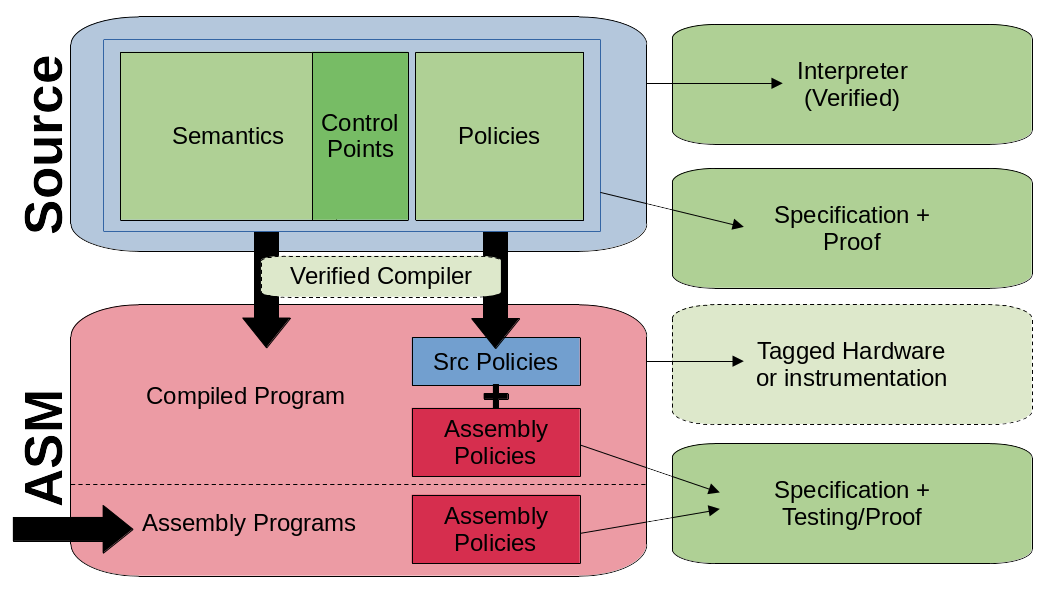
\includegraphics[width=\textwidth]{Structure.png}
  \caption{Tagging with Source Language}
  \label{fig:language}
\end{figure}

\section{Overview}

This dissertation is divided into three main parts. The first proposes a new formal characterization
of stack safety using concepts from language-based security. Stack safety exemplifies the challenges
of specifying a policy: ``the stack'' is not a clearly defined language concept, but a loosely
defined component of a system's ABI that is relied on by many different higher-level abstractions.
Performance tradeoffs are relevant as well: the ``lazy'' stack safety policies studied by
Roessler and DeHon~\cite{RoesslerD18} permit functions to write into one another's
frames, intuitively a violation, but taint the written locations so that their owner cannot
access them later. No prior characterization of stack safety captures this style of safety.

The second part presents Tagged C, a \emph{source-level} specification framework that allows
engineers to describe policies in terms of familiar C-level concepts. Tagged C addresses the
challenges in definition, specification, and validation that relate to assembly-level programs.
It takes the form of a variant C language whose semantics is parameterized by tags
attached to its data and rules that triggered during execution at a set of predefined
\emph{control points}. Control points correspond to significant execution events, such as
function calls, expression evaluation, and pointer-based memory accesses.

Tagged C allows policies to be defined at the source level via a fixed interface
that never requires rewriting code. Where assembly instructions can serve different roles and must
be distinguished for tag purposes, each Tagged C control point serves one clear role. The policy
designer needs little knowledge of how the control points might be compiled, and need not
deal with portions of a policy that would be colored red in Figure \ref{ex:call}.

The current iteration of Tagged C is implemented as an interpreter, based on that of
CompCert C \cite{Leroy09:CompCert}. This is sufficient to test small programs. Ultimately
Tagged C will be compiled to a PIPE target by injecting the source policy's tag rules
as a payload into a predefined assembly-level policy that handles the bookkeeping.

The Tagged-C semantics (also based on CompCert C) gives a formal definition of what each
control point does. This means that properties of a policy may be proven in terms of how
source programs behave when run under it. Just as it is far preferable to prove properties
of a program with regard to its source semantics, this is a major step forward for policy
verification.

The final third of this dissertation makes use of Tagged C to perform a source-level specification and
verification of a novel compartmentalization property. The specification takes the form of
an abstract semantics that is compartmentalized by construction. This compartmentalized semantics
is written to keep compartments' local data isolated entirely in separate address spaces.
Both the specification and the policy that enforces it are novel, and improve upon the
state-of-the art in tag-based compartmentalization by allowing objects to be shared between
compartments via passed pointers, without the overhead of protecting every object individually.
The proof is mechanized. The policy definition, its
specification, and its proof are all concrete contributions on their own, and together they
serve to demonstrate that Tagged C is a suitable setting in which to perform the entire
define-specify-validate sequence.

\subsection{Contributions and Organization}

Chapter \ref{ch:background} introduces the concept of tag-based reference monitors
and brings the reader up to date on the state-of-the-art in that and related areas.
The contributions in this dissertation are divided across its three main topics.

\paragraph{Stack Safety}

Chapter \ref{ch:stacksafety} gives a novel formalization of stack safety in the
form of a collection of trace properties. Our contributions are:

\begin{itemize}
  \item A novel characterization of stack safety as a conjunction
        of security properties: confidentiality and integrity for callee
        and caller, plus well-bracketed control-flow.
        The properties are parameterized over a notion of
        external observation, allowing them to characterize lazy enforcement
        mechanisms.
  \item An extension of these core definitions to
        describe a realistic setting with argument passing on the stack,
        callee-saves registers, and tail-call elimination. The model is
        modular enough that adding these features is straightforward.
  \item Validation of a published enforcement mechanism,
        \emph{Lazy Tagging and Clearing}, via property-based random testing; we find that
        it falls short, and propose and validate a fix.
\end{itemize}

This chapter was first published at the IEEE Computer Security Foundations Symposium,
July 2023 as ``Formalizing Stack Safety as a Security Policy,'' a
joint work with Roberto Blanco, Leonidas Lampropoulos, Benjamin Pierce, and Andrew Tolmach
\cite{Anderson23:StackSafety}.

\paragraph{Tagged C}

In Chapter \ref{ch:taggedc}, we attack the definition problem by lifting tagged enforcement
to the level of C source code. We introduce Tagged C, a C variant whose semantics are parameterized
by an arbitrary tag-based policy. Our contributions are:

\begin{itemize}
\item The design of a comprehensive set of {\em control points} at which the C language interfaces
  with a tag-based policy. These expand on prior work by encompassing the full C language
  while being powerful enough to enable a range of policies even in the presence of C's more
  challenging constructs (e.g., {\tt goto}, conditional expressions, etc.).
\item Tagged C policies enforcing: (1) compartmentalization;
  (2) memory safety, with realistic memory models that support varying kinds of low-level idioms;
  and (3) secure information flow.
\item A full formal semantic definition for Tagged C, formalized in Coq, describing how the
  control points interact with programs, and an interpreter, implemented and verified against
  the semantics in Coq and extracted to OCaml.
\end{itemize}

The core of this chapter was first published at the International Conference on Runtime Verification,
October 2023 as ``Flexible Runtime Security Enforcement with Tagged C,'' a joint work
with Andrew Tolmach and Allison Naaktgeboren \cite{Anderson23:TaggedC}. Some technical
details are also published in Chhak et al. \cite{}, a joint work with CHR Chhak and Andrew Tolmach.
The original content has been updated to reflect further development, and the chapter has been
extended with a detailed discussion of the design decisions that inform the current development.

\paragraph{Compartmentalization}

Finally, I return to the specification and validation problems, now at the C level. Chapter
\ref{ch:compartments} presents a compartmentalization policy in conjunction with the abstract
compartmentalization scheme that it enforces, and proves that the policy indeed enforces the
abstract model. The detailed contributions are:

\begin{itemize}
\item A formal model of C compartmentalization in the form of an abstract machine that
  supports sharing between compartments while keeping their memories isolated by construction.
\item A novel compartmentalization policy for Tagged C that supports cross-compartment
  sharing with fewer constraints on available tags than similar systems from the literature.
\item A proof that the compartmentalization policy is safe with respect to the abstract semantics.
\end{itemize}

This work is not yet submitted for publication.

\chapter{Tags and Monitors}
\label{ch:background}

\chapter{Formalizing Stack Safety as a Security Policy}
\label{ch:stacksafety}

\chapter{Flexible Runtime Security Enforcement with Tagged C}
\label{ch:taggedc}

\chapter{Formalizing Compartmentalization as an Abstract Machine}
\label{ch:compartments}

\chapter{Conclusion}

\bibliographystyle{acm}
\bibliography{taggedc.bib}

\end{document}
